% !TEX encoding = UTF-8 Unicode
\documentclass[10pt,aspectratio=169,]{beamer}
\setbeamercovered{transparent=10}
\usetheme[
%  showheader,
%  red,
  purple,
%  gray,
%  graytitle,
  colorblocks,
%  noframetitlerule,
]{Verona}

\usepackage[T1]{fontenc}
\usepackage[utf8]{inputenc}
\usepackage{lipsum}
%%%%%%%%%%%%%%%%%%%%%%%%%%%%%%%
% Mac上使用如下命令声明隶书字体，windows也有相关方式，大家可自行修改
%\providecommand{\lishu}{\CJKfamily{zhli}}
%%%%%%%%%%%%%%%%%%%%%%%%%%%%%%%
\usepackage{multicol}
\usepackage{tikz}
\usetikzlibrary{fadings,positioning,arrows.meta,shapes.geometric,calc}
%
%\setbeamertemplate{sections/subsections in toc}[ball]
\usepackage{xeCJK}
\usepackage{ctex, hyperref}
\usepackage{fontspec}
\usepackage{listings}
\usepackage{caption}
\usepackage{subcaption}
\usefonttheme{professionalfonts}
\def\mathfamilydefault{\rmdefault}
\usepackage{amsmath}
\usepackage{multirow}
\usepackage{booktabs}
\usepackage{bm}
\usepackage[ruled,linesnumbered]{algorithm2e}
\usepackage{listings}
\graphicspath{{./}{../paper/images/}}
\setbeamertemplate{section in toc}{\hspace*{1em}\inserttocsectionnumber.~\inserttocsection\par}
\setbeamertemplate{subsection in toc}{\hspace*{2em}\inserttocsectionnumber.\inserttocsubsectionnumber.~\inserttocsubsection\par}
\setbeamerfont{subsection in toc}{size=\small}
\AtBeginSection[]{
	\begin{frame}%
        \begin{multicols}{2}%分列两栏的目录
		    \frametitle{Outline}%
		    \kaishu{\textbf{\tableofcontents[currentsection]}}
        \end{multicols}
	\end{frame}
}
%\AtBeginSubsection[]{%
%	\begin{frame}%
%		\frametitle{Outline}%
%		\textbf{\tableofcontents[currentsection, currentsubsection]} %
%	\end{frame}%
%}
\title{基于混合检索器的多模态生成模型研究与实现}
\subtitle{中期答辩}
\author[时子延]{时子延}
\mail{\url{19220422}}
\institute[19220422]{指导老师: 宋歌\\计算机与电子信息学院/人工智能学院\\南京师范大学}
\date{\today}
\titlegraphic[width=3cm]{nnu_big_logo}{}


% 配置 listings 包的一些基本样式
\lstset{
	basicstyle=\ttfamily\small,
	keywordstyle=\color{blue},
	stringstyle=\color{red},
	commentstyle=\color{green},
	morecomment=[l][\color{magenta}]{\#},
	frame=single,
	breaklines=true,
  postbreak=\mbox{\textcolor{red}{$\hookrightarrow$}\space},
}
%%%%%%%%%%%%%%%%%%%%%%%%%%%%%%%%
% ----------- 标题页 ------------
%%%%%%%%%%%%%%%%%%%%%%%%%%%%%%%%

\begin{document}

\maketitle

%%%%%%%%%%%%%%%%%%%%%%%%%%%%%%%%
% ----------- FRAME ------------
%%%%%%%%%%%%%%%%%%%%%%%%%%%%%%%%

\section{研究概述}
\subsection{研究目的}
\begin{frame}{研究概述}
	\framesubtitle{研究目的}
	\begin{block}{研究目标}
		\begin{itemize}
			\item 面向多模态检索增强生成（mRAG）场景，提升检索器返回有效视觉证据的能力。
			\item 基于 MRAG-Bench 构建统一评测流程，回答“更懂指令的检索器是否真的能提升下游问答效果”。
			\item 以 MagicLens 为核心检索器，对比 GT Oracle、Random、Text-only 与 corpus 检索等策略。
		\end{itemize}
	\end{block}
	\begin{alertblock}{挑战}
		\begin{itemize}
			\item 多模态问答中，性能瓶颈究竟在“候选从哪里来”，还是“候选如何排序”。
			\item 当问题真正依赖视觉证据时，现有检索器是否能稳定召回并利用正确图像。
		\end{itemize}
	\end{alertblock}
\end{frame}

\subsection{意义与现状}
\begin{frame}{研究概述}
	\framesubtitle{本课题的目的及研究意义}
	\begin{columns}[T]
		\begin{column}{0.54\textwidth}
			\begin{block}{研究动机}
				\begin{itemize}
					\item LLM/MLLM 仍存在知识冻结与幻觉问题，RAG 通过外部知识缓解真实性问题。
					\item 在多模态场景下，错误不仅是“文本事实编造”，还包括“视觉事实编造”。
					\item 因此需要从文本 RAG 走向 mRAG，并重点提升视觉证据检索质量。
				\end{itemize}
			\end{block}
		\end{column}
		\begin{column}{0.42\textwidth}
			\begin{alertblock}{研究意义}
				\begin{itemize}
					\item 为具身智能提供可检索的长期记忆与证据链。
					\item 为脑机接口与高可靠辅助沟通提供更低幻觉的检索基础。
					\item 为后续检索器训练与扩散模型驱动增强提供实验基础。
				\end{itemize}
			\end{alertblock}
		\end{column}
	\end{columns}
\end{frame}

\begin{frame}{研究概述}
	\framesubtitle{本课题的国内外研究现状}
	\begin{block}{mRAG 研究主线}
		\begin{itemize}
			\item 框架层：mRAG 从静态单轮走向动态、按需、多轮检索，核心关注幻觉抑制与时效性提升。
			\item 表示层：CLIP、ALIGN 等统一语义空间方法推动跨模态检索成为可能。
			\item 检索层：FG-CLIP、Long-CLIP、MagicLens 等工作分别从细粒度理解、长文本建模、开放式指令检索改进效果。
		\end{itemize}
	\end{block}
	\begin{alertblock}{目前仍存在的空缺}
		\begin{itemize}
			\item 现有研究更关注通用框架综述，缺少面向“视觉证据是否真正被找对”的系统评测。
			\item 多数实验没有拆开粗召回与重排两类能力，难以定位 mRAG 的真实瓶颈。
		\end{itemize}
	\end{alertblock}
\end{frame}

\begin{frame}{研究概述}
	\framesubtitle{MRAG-Bench 数据集定位}
	\begin{columns}[T]
		\begin{column}{0.58\textwidth}
			\begin{figure}[htbp]
				\centering
				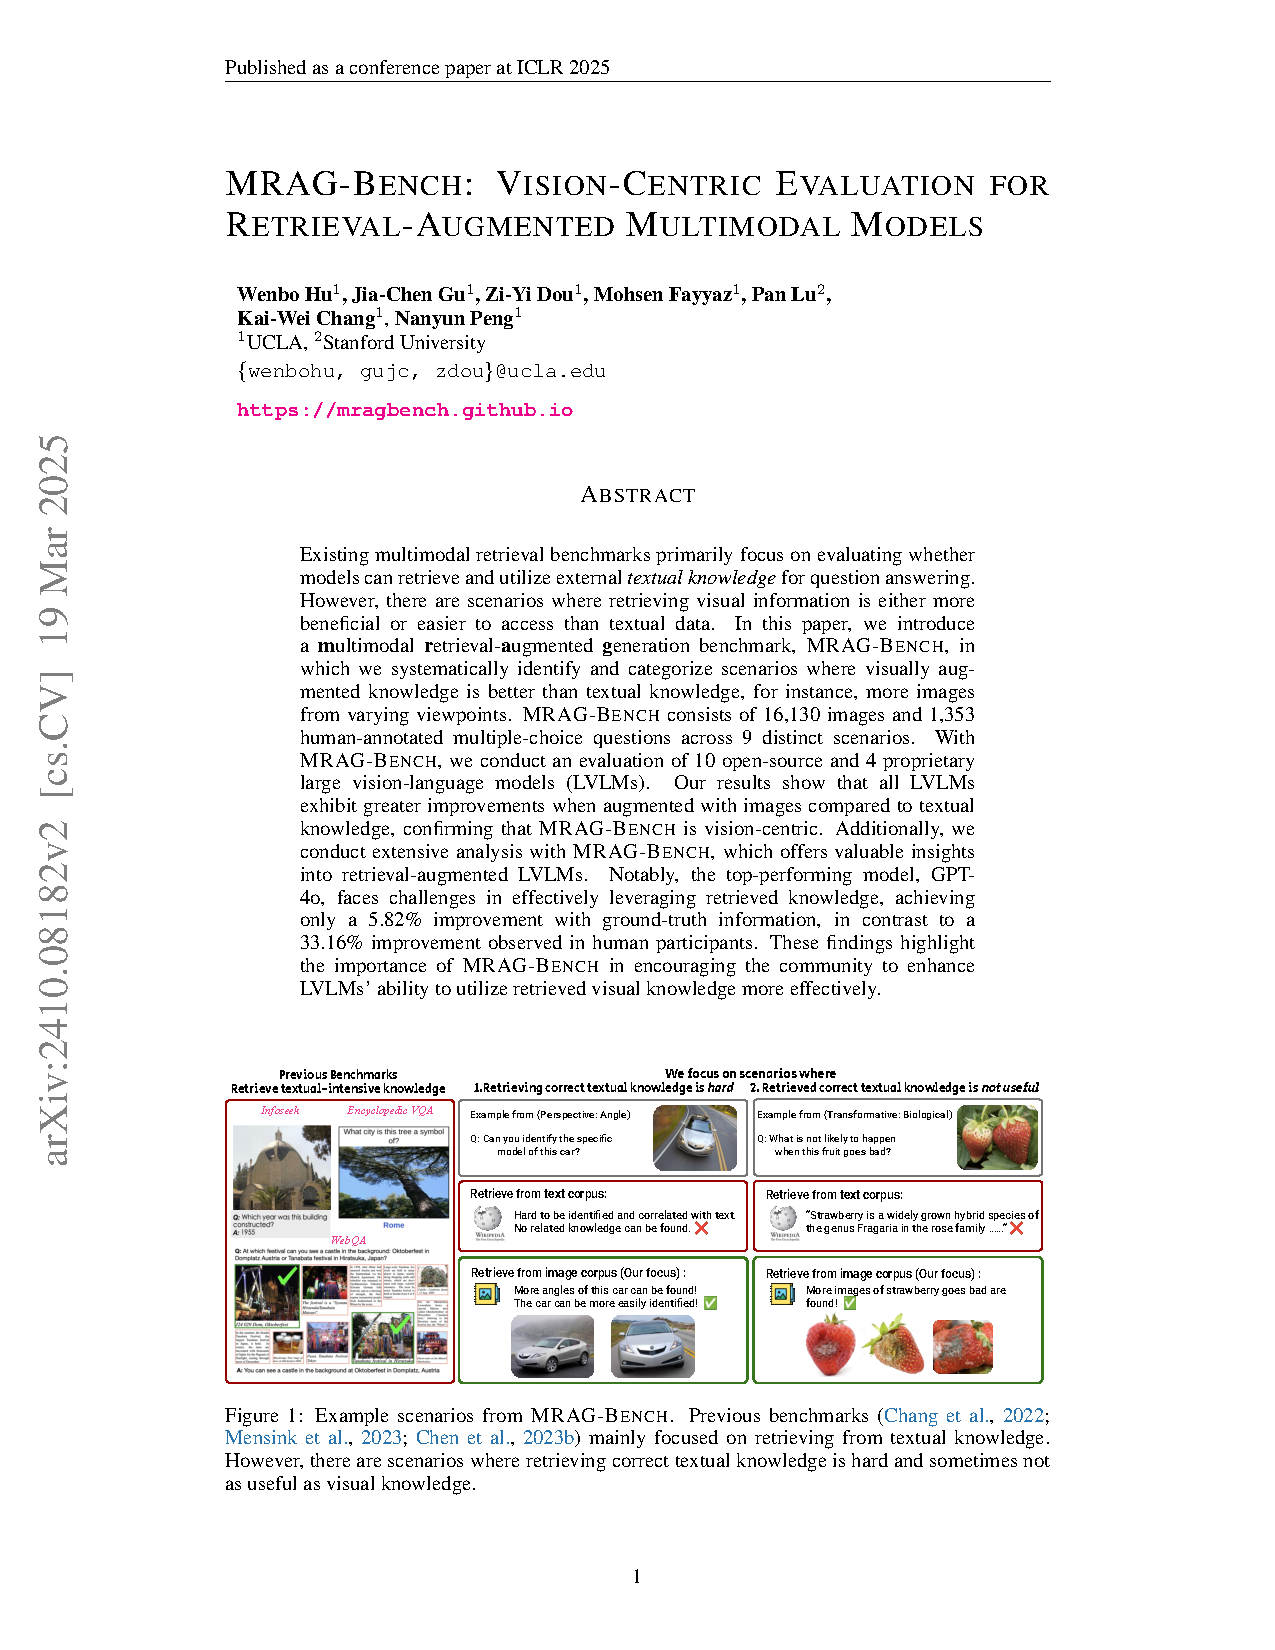
\includegraphics[page=1,width=\linewidth]{../doc/2410.08182v2.pdf}
			\end{figure}
		\end{column}
		\begin{column}{0.38\textwidth}
			\begin{block}{出发点}
				\begin{itemize}
					\item MRAG-Bench 是 vision-centric benchmark。
					\item 核心问题不是“能否检索文本知识”，而是“视觉证据是否比文本更关键”。
					\item 这与本文从图像检索器切入 mRAG 的研究目标直接一致。
				\end{itemize}
			\end{block}
		\end{column}
	\end{columns}
\end{frame}

\begin{frame}{研究概述}
	\framesubtitle{MRAG-Bench 场景与样例}
	\begin{columns}[T]
		\begin{column}{0.46\textwidth}
			\begin{figure}[htbp]
				\centering
				\includegraphics[page=3,width=\linewidth]{../doc/2410.08182v2.pdf}
			\end{figure}
		\end{column}
		\begin{column}{0.50\textwidth}
			\begin{figure}[htbp]
				\centering
				\includegraphics[page=4,width=\linewidth]{../doc/2410.08182v2.pdf}
			\end{figure}
		\end{column}
	\end{columns}
\end{frame}

\section{研究内容与方法}
\subsection{研究内容}
\begin{frame}{研究内容与方法}
	\framesubtitle{本课题的研究内容}
	\begin{columns}[T]
		\begin{column}{0.54\textwidth}
			\begin{block}{研究内容}
				\begin{enumerate}
					\item 基于 MRAG-Bench 重构视觉证据导向的 mRAG 评测任务，将检索阶段作为核心变量。
					\item 引入 MagicLens 作为多模态检索器，研究其在“关系驱动证据检索”中的实际价值。
					\item 设计 GT Oracle、Random、Retrieved-Rerank、Corpus-CLIP 等对照实验，量化不同检索策略的收益与上限。
				\end{enumerate}
			\end{block}
		\end{column}
		\begin{column}{0.42\textwidth}
			\begin{alertblock}{组织思路}
				\begin{itemize}
					\item 从整体准确率、分场景准确率、GT 覆盖率与失败模式四个层面分析检索器表现。
					\item 将实验明确拆为 \textbf{Rerank line} 和 \textbf{Corpus line}。
					\item 分别回答排序收益与粗召回收益。
				\end{itemize}
			\end{alertblock}
		\end{column}
	\end{columns}
\end{frame}

\begin{frame}{研究内容与方法}
	\framesubtitle{MagicLens 模型动机}
	\begin{columns}[T]
		\begin{column}[T]{0.41\textwidth}
			\scriptsize
			\begin{block}{为什么引入 MagicLens}
				\begin{itemize}
					\item 传统图像检索更偏向视觉相似性，难表达“内部视角”“相关物品”“不同时刻”等开放关系。
					\item MagicLens 将检索定义为 $(image_q,\ instruction)\rightarrow image_t$，强调关系驱动的目标搜索。
					\item 这与 MRAG-Bench 中大量依赖视觉证据与跨图关系的题型高度契合。
				\end{itemize}
			\end{block}
			\begin{alertblock}{论文要点}
				\begin{itemize}
					\item 开放式 instruction 让检索从“像不像”转向“关系是否匹配”。
					\item MagicLens 在多类检索 benchmark 上表现稳定，同时保持较好的参数效率。
				\end{itemize}
			\end{alertblock}
		\end{column}
		\begin{column}[T]{0.55\textwidth}
			\vspace{-1.2em}
			\centering
			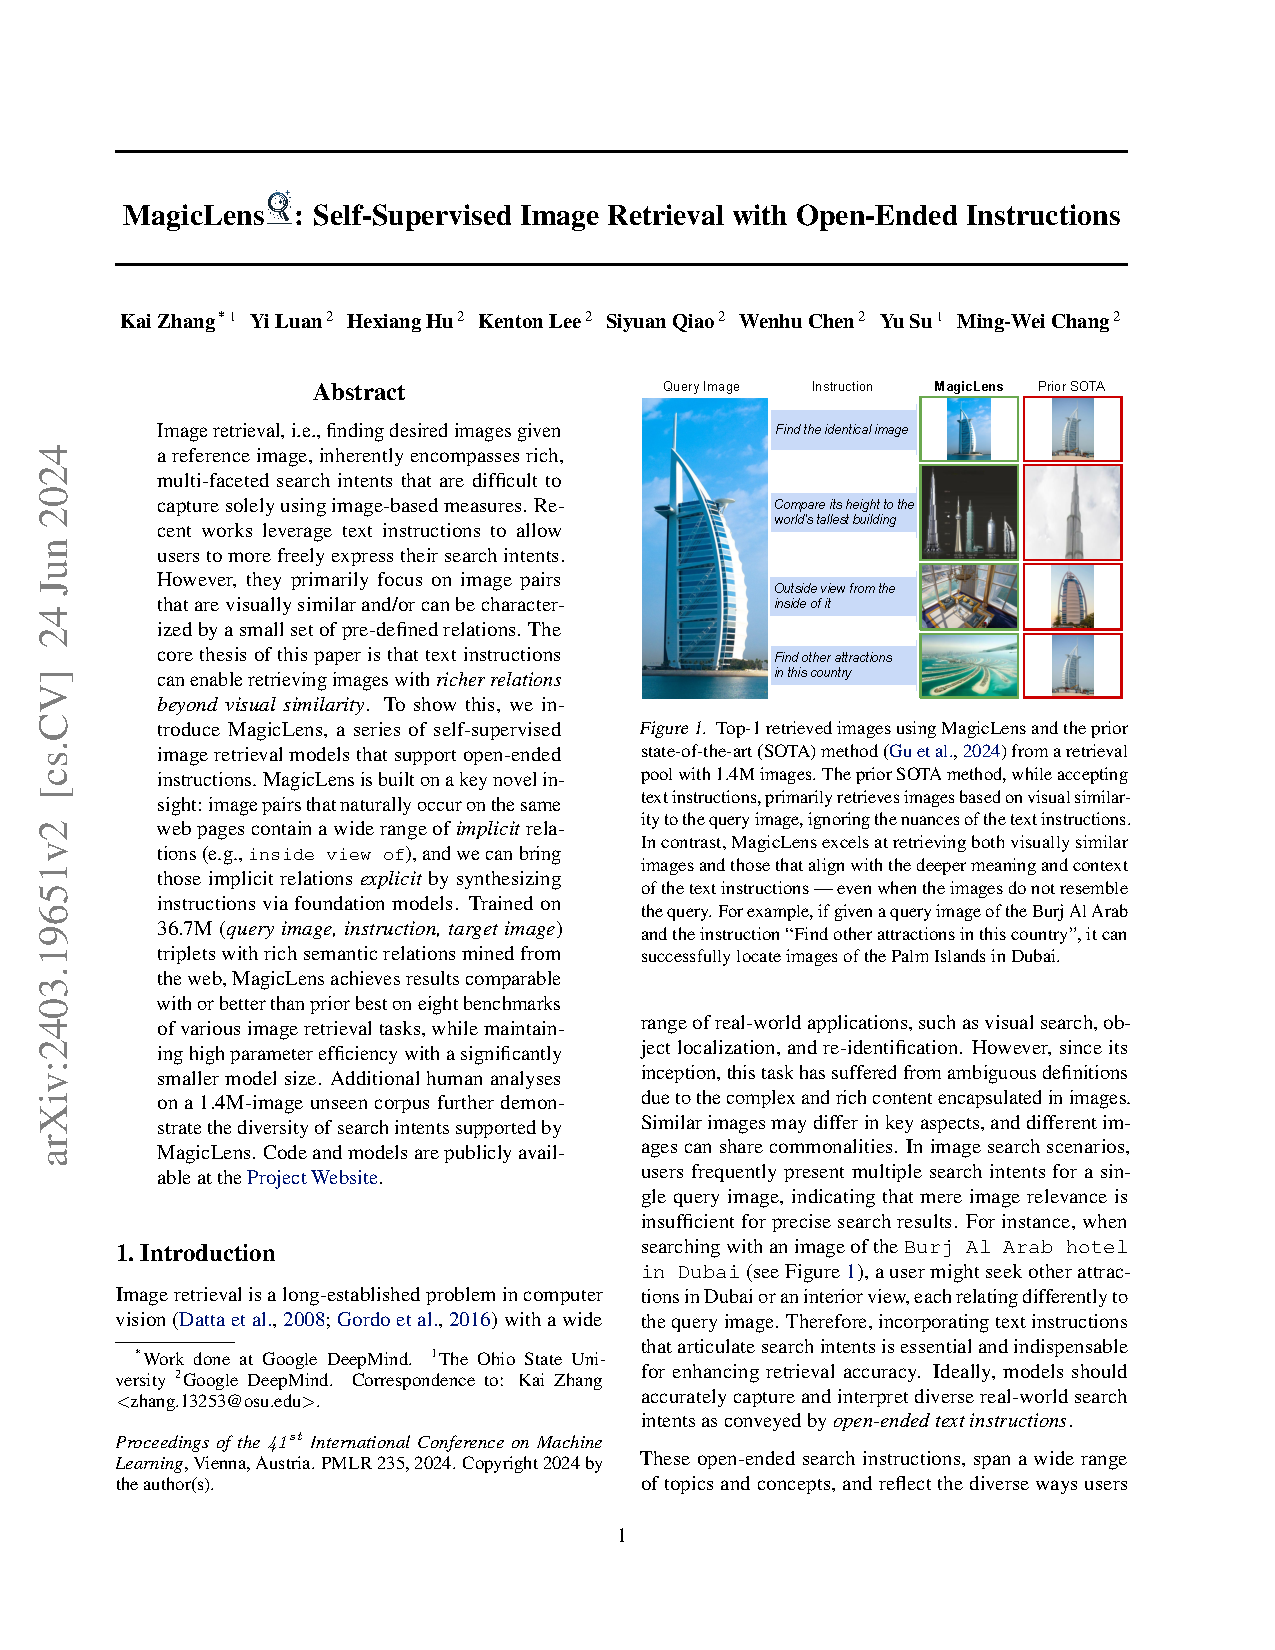
\includegraphics[page=1,height=0.72\textheight,keepaspectratio]{../doc/magiclens.pdf}
		\end{column}
	\end{columns}
\end{frame}

\begin{frame}{研究内容与方法}
	\framesubtitle{MagicLens 训练数据与模型结构}
	\begin{columns}[T]
		\begin{column}[T]{0.45\textwidth}
			\scriptsize
			\begin{block}{自监督数据构造}
				\begin{itemize}
					\item 从同一网页中挖掘自然共现图像对，而不是只依赖人工定义关系。
					\item 用 LMM/LLM 为图像对生成开放式 instruction，形成 $(query\ image,\ instruction,\ target\ image)$ 三元组。
					\item 最终构建约 3670 万条训练样本，覆盖大量隐式语义关系。
				\end{itemize}
			\end{block}
			\begin{alertblock}{模型结构}
				\begin{itemize}
					\item 共享参数的 dual-encoder，以 CLIP/CoCa 为初始化。
					\item 通过 self-attention 融合图像与指令，再用 attention pooling 压缩成单向量表示。
					\item target 端使用 $(image_t,\ "")$ 编码，并采用 contrastive loss；同时把 query image 本身作为 hard negative。
				\end{itemize}
			\end{alertblock}
		\end{column}
		\begin{column}[T]{0.51\textwidth}
			\vspace{-1.2em}
			\centering
			\includegraphics[page=4,height=0.72\textheight,keepaspectratio]{../doc/magiclens.pdf}
		\end{column}
	\end{columns}
\end{frame}

\subsection{技术路线}
\begin{frame}{研究内容与方法}
	\framesubtitle{实验设计与技术路线}
	\begin{columns}[T]
		\begin{column}{0.48\textwidth}
			\begin{block}{统一评测流程}
				\begin{enumerate}
					\item 输入 query image + question
					\item 检索 Top-$k$ 候选图像
					\item 将问题与候选图送入 LLaVA
					\item 输出多项选择答案并统计指标
				\end{enumerate}
			\end{block}
		\end{column}
		\begin{column}{0.48\textwidth}
			\begin{alertblock}{对照设置}
				\begin{itemize}
					\item E0: LLaVA + GT-RAG baseline
					\item E1/E2: 固定候选集上的 MagicLens rerank
					\item E3: CLIP 从完整 corpus 召回 Top-5
					\item E6: CLIP 粗召回 + MagicLens 重排
					\item E7: MagicLens 直接从完整 corpus 召回
				\end{itemize}
			\end{alertblock}
		\end{column}
	\end{columns}
	\vspace{0.5em}
	\begin{block}{评价指标}
		整体 Accuracy、九类场景分布、GT 覆盖率、接近 Oracle 的程度，以及“检索对但生成错 / 检索错但生成对”的失败模式。
	\end{block}
\end{frame}

\begin{frame}{研究内容与方法}
	\framesubtitle{模型架构图}
	\centering
	\begin{tikzpicture}[
		x=1cm,y=1cm,
		>={Latex[length=3mm]},
		box/.style={rounded corners=3pt, minimum width=2.15cm, minimum height=0.9cm, align=center, font=\small\bfseries, text=white},
		data/.style={box, fill=structure.fg!88},
		model/.style={box, fill=black!72},
		aux/.style={box, fill=nnucolor!78!black},
		note/.style={rounded corners=2pt, draw=black!18, fill=black!3, minimum width=2.3cm, minimum height=0.62cm, align=center, font=\scriptsize},
		line/.style={thick, draw=black!65},
		hl/.style={thick, draw=red!70}
	]
		\node[data] (query) at (0,0) {Query Image\\+ Question};
		\node[data] (corpus) at (0,-2.1) {Image Corpus};
		
		\node[model] (clip) at (3.2,-0.9) {CLIP\\Retriever};
		\node[aux] (magiclens) at (6.25,-0.9) {MagicLens\\Reranker};
		\node[model] (llava) at (9.3,-0.9) {LLaVA};
		\node[data] (answer) at (12.1,-0.9) {MCQA\\Answer};
		
		\node[note] (topk) at (3.2,0.7) {Top-$K$ candidates};
		\node[note] (reordered) at (6.25,0.7) {reordered evidence};
		\node[note] (baseline) at (3.2,-2.35) {E3: direct corpus retrieval};
		\node[note] (hybrid) at (6.25,-2.35) {E6: retrieval + rerank};
		\node[note] (directml) at (6.25,-3.15) {E7: MagicLens direct retrieval};
		
		\draw[line,->] (query) -- (clip);
		\draw[line,->] (corpus) -- (clip);
		\draw[line,->] (clip) -- (magiclens);
		\draw[line,->] (magiclens) -- (llava);
		\draw[line,->] (llava) -- (answer);
		
		\draw[line,->] ($(clip.north)+(0,0.1)$) -- (topk.south);
		\draw[line,->] ($(magiclens.north)+(0,0.1)$) -- (reordered.south);
		
		\draw[hl,->,rounded corners=3pt] ($(clip.south)+(0,-0.15)$) |- ($(llava.south)+(0,-0.15)$);
		\node[font=\scriptsize, text=red!70!black] at (6.2,-1.85) {baseline path};
		
		\draw[draw=structure.fg!25, rounded corners=5pt, line width=0.8pt] (-1.2,1.4) rectangle (13.2,-3.55);
	\end{tikzpicture}
	\vspace{0.25em}
	\scriptsize
	\begin{columns}[T]
		\begin{column}{0.31\textwidth}
			\begin{block}{E3}
				CLIP 直接从完整 corpus 召回 Top-$K$ 候选。
			\end{block}
		\end{column}
		\begin{column}{0.31\textwidth}
			\begin{alertblock}{E6}
				CLIP 粗召回后，再用 MagicLens 重排。
			\end{alertblock}
		\end{column}
		\begin{column}{0.31\textwidth}
			\begin{block}{E7}
				MagicLens 直接作为全库 retriever。
			\end{block}
		\end{column}
	\end{columns}
\end{frame}

\begin{frame}{研究内容与方法}
	\framesubtitle{任务定义与损失函数}
	\begin{columns}[T]
		\begin{column}{0.48\textwidth}
			\begin{block}{任务定义}
				\begin{equation*}
					Q=(x_q,q)
				\end{equation*}
				\begin{equation*}
					I=R(Q)=\{i_1,\dots,i_K\}
				\end{equation*}
				\begin{equation*}
					\hat{y}=M(Q,I)
				\end{equation*}
			\end{block}
			\begin{alertblock}{排序分数}
				\begin{equation*}
					s_i=\langle z_q,z_i\rangle
				\end{equation*}
			\end{alertblock}
		\end{column}
		\begin{column}{0.48\textwidth}
			\begin{block}{排序损失}
				\begin{equation*}
				\mathcal{L}_{\text{rank}}
				=
				-\log
				\frac{\exp(s(q,i^+))}
				{\sum_j \exp(s(q,i_j))}
				\end{equation*}
			\end{block}
			\begin{alertblock}{联合优化目标}
				\begin{equation*}
				\mathcal{L}_{\text{ans}}
				=
				-\log p(\hat{y}=y^\ast \mid Q,I)
				\end{equation*}
				\begin{equation*}
				\mathcal{L}
				=
				\mathcal{L}_{\text{rank}}
				+
				\lambda \mathcal{L}_{\text{ans}}
				\end{equation*}
			\end{alertblock}
		\end{column}
	\end{columns}
\end{frame}

\section{研究进度与结果}
\subsection{研究进度}
\begin{frame}{研究进度与结果}
	\framesubtitle{研究进度}
	\begin{block}{已完成}
		\begin{itemize}
			\item 搭建 MRAG-Bench 数据与评测管线，明确图像候选进入模型的真实规则。
			\item 跑通 GT-RAG、Retrieved-Rerank、CLIP corpus Top-5 等基线实验。
			\item 完成候选重叠统计与问题拆分，明确区分 rerank 与 corpus 两条实验线。
		\end{itemize}
	\end{block}
	\begin{alertblock}{正在进行}
		\begin{itemize}
			\item 集成 MagicLens 到完整 corpus 检索流程，形成 E6 主实验。
			\item 新增 E7 直检索实验脚本，用于评估 MagicLens 作为 direct retriever 的效果。
			\item 分场景分析检索收益，定位 Temporal、Scope、Incomplete 等难点场景。
		\end{itemize}
	\end{alertblock}
\end{frame}

\subsection{阶段结果}
\begin{frame}{研究进度与结果}
	\framesubtitle{研究结果一：数据集与候选分析}
	\begin{columns}[T]
		\begin{column}{0.52\textwidth}
			\begin{block}{MRAG-Bench 数据特征}
				\begin{itemize}
					\item 共 1353 个测试样本，覆盖 9 类视觉证据依赖场景。
					\item GT 候选平均 4.70 张，\texttt{retrieved\_images} 原始字段固定为 5 张。
					\item Incomplete 场景在 dataloader 中会被截断为 1 张，需单独分析。
				\end{itemize}
			\end{block}
		\end{column}
		\begin{column}{0.44\textwidth}
			\begin{alertblock}{重叠统计结论}
				\begin{itemize}
					\item 44.12\% 样本中，retrieved 与 GT 完全无重叠。
					\item 平均 GT 覆盖率仅 22.78\%。
					\item 说明数据集自带候选与 oracle 候选存在显著偏差。
				\end{itemize}
			\end{alertblock}
		\end{column}
	\end{columns}
	\vspace{0.4em}
	\centering
	\scriptsize
	\begin{tabular}{lccc}
		\toprule
		Source & 1 张 & 5 张 & Avg. \\
		\midrule
		GT raw & 102 & 1251 & 4.70 \\
		Retrieved raw & 0 & 1353 & 5.00 \\
		Retrieved effective & 102 & 1251 & 4.70 \\
		\bottomrule
	\end{tabular}
\end{frame}

\begin{frame}{研究进度与结果}
	\framesubtitle{研究结果：候选分布可视化}
	\begin{columns}[T]
		\begin{column}{0.60\textwidth}
			\begin{figure}[htbp]
				\centering
				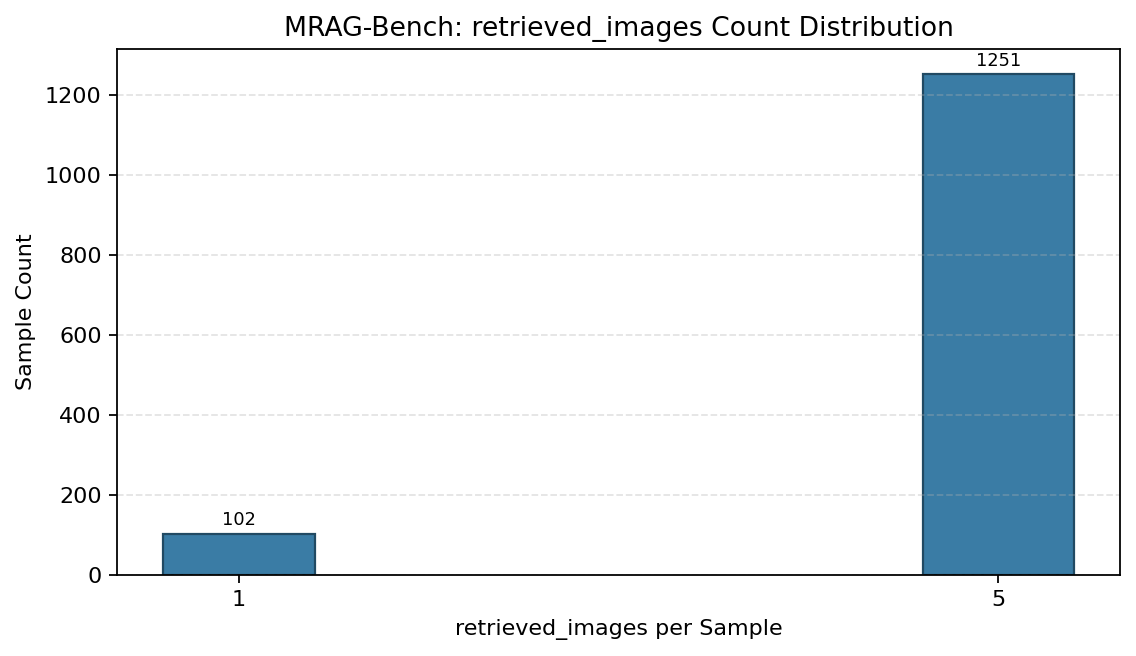
\includegraphics[width=\linewidth]{retrieved_images_hist.png}
			\end{figure}
		\end{column}
		\begin{column}{0.36\textwidth}
			\begin{block}{观察}
				\begin{itemize}
					\item 数据集给定候选与 GT 候选分布并不一致。
					\item 一部分样本中，retrieved 候选几乎不覆盖真正有效证据。
					\item 这也是本文把局部 rerank 与全库检索分开讨论的直接原因。
				\end{itemize}
			\end{block}
		\end{column}
	\end{columns}
\end{frame}

\begin{frame}{研究进度与结果}
	\framesubtitle{E0-E7 含义与评价指标}
	\begin{columns}[T]
		\begin{column}{0.48\textwidth}
			\begin{block}{实验线含义}
				\begin{itemize}
					\item E0：GT-RAG，上界参考。
					\item E1：GT 候选 + MagicLens rerank，测排序收益。
					\item E2：数据集候选 + MagicLens rerank，测局部重排能力。
					\item E3：CLIP 全库直检索，测粗召回 baseline。
					\item E4：No-RAG，测无外部证据基线。
					\item E5：GT 候选但关闭 rerank，用于隔离 E1 的排序收益。
					\item E6：CLIP 粗召回 + MagicLens rerank，测混合检索。
					\item E7：MagicLens 全库直检索，测 direct retriever 能力。
				\end{itemize}
			\end{block}
		\end{column}
		\begin{column}{0.48\textwidth}
			\begin{alertblock}{指标在回答什么}
				\begin{itemize}
					\item Overall Accuracy：最终问答效果。
					\item 分场景 Accuracy：不同视觉证据类型下的稳定性。
					\item E1 vs E5：判断 rerank 是否真正带来收益。
					\item E3 vs E6：判断重排能否改善 CLIP 粗召回。
					\item E3 vs E7：判断 MagicLens 是否适合直接做全库召回。
					\item E4 vs 其余实验：判断“给证据”是否真的优于“不给证据”。
				\end{itemize}
			\end{alertblock}
		\end{column}
	\end{columns}
\end{frame}

\begin{frame}{研究进度与结果}
	\framesubtitle{研究结果二：阶段性实验表现}
	\begin{columns}[T]
		\begin{column}{0.58\textwidth}
			\begin{block}{Overall 对照}
				\centering
				\tiny
				\resizebox{0.98\linewidth}{!}{
				\begin{tabular}{lll}
					\toprule
					Track & Method & Overall (\%) \\
					\midrule
					Control & E0: GT-RAG & 59.05 \\
					Rerank & E1: GT+ML rerank & 60.16 \\
					Rerank & E2: Ret+ML rerank & 51.74 \\
					Corpus & E3: CLIP corpus & 50.41 \\
					Control & E4: No-RAG & 53.14 \\
					Control & E5: GT no rerank & 60.16 \\
					Corpus & E6: CLIP+ML rerank & 50.33 \\
					Corpus & E7: ML corpus & 47.97 \\
					\bottomrule
				\end{tabular}
				}
			\end{block}
		\end{column}
		\begin{column}{0.38\textwidth}
			\scriptsize
			\begin{block}{初步观察}
				\begin{itemize}
					\item E1 与 E5 接近，GT 条件下 rerank 收益有限。
					\item E4 高于 E3/E6/E7，说明噪声证据可能伤害回答。
					\item E6 与 E3 接近，重排尚未稳定改善粗召回。
					\item E7 低于 E3，MagicLens 直检索仍弱于 CLIP。
				\end{itemize}
			\end{block}
		\end{column}
	\end{columns}
	\vspace{0.2em}
	\begin{alertblock}{分场景现象}
		E4 在 Incomplete 上达到 33.33\%，明显高于 E3 的 22.55\%；E6 在 Scope 和 Incomplete 上高于 E3，但在 Partial、Occlusion 与 Biological 上下降，说明当前提升并不稳定。
	\end{alertblock}
\end{frame}

\begin{frame}{研究进度与结果}
	\framesubtitle{研究结果：E7 直检索实验}
	\begin{columns}[T]
		\begin{column}{0.44\textwidth}
			\begin{block}{E7 核心结果}
				\begin{itemize}
					\item 任务：MagicLens 直接从完整 corpus 召回 Top-5。
					\item Overall Accuracy：47.97\%（649/1353）。
					\item 对比 E3：低于 CLIP corpus baseline 的 50.41\%。
				\end{itemize}
			\end{block}
		\end{column}
		\begin{column}{0.52\textwidth}
			\centering
			\scriptsize
			\begin{tabular}{lcc}
				\toprule
				Scenario & E3 & E7 \\
				\midrule
				Angle & 52.48 & 51.55 \\
				Partial & 54.07 & 47.56 \\
				Scope & 48.04 & 45.10 \\
				Occlusion & 54.63 & 48.15 \\
				Temporal & 46.31 & 46.98 \\
				Deformation & 58.82 & 50.00 \\
				Incomplete & 22.55 & 32.35 \\
				Biological & 50.00 & 50.98 \\
				Others & 57.50 & 51.67 \\
				\bottomrule
			\end{tabular}
		\end{column}
	\end{columns}
	\vspace{0.4em}
	\begin{alertblock}{初步判断}
		E7 说明 MagicLens 可以直接承担全库召回，但当前整体稳定性仍不如 CLIP；不过它在 Incomplete 场景上有明显优势，说明其在结构缺失类问题上存在潜力。
	\end{alertblock}
\end{frame}

\begin{frame}{研究进度与结果}
	\framesubtitle{全实验结果总表说明}
	\begin{columns}[T]
		\begin{column}{0.48\textwidth}
			\begin{block}{Control / Rerank}
				\begin{itemize}
					\item E0：LLaVA + GT-RAG baseline，作为较高上界。
					\item E1：在 GT 候选集上做 MagicLens rerank。
					\item E2：在数据集给定候选上做 MagicLens rerank。
					\item E4：LLaVA + No-RAG，对应无外部知识基线。
					\item E5：GT 候选输入，但关闭 MagicLens 重排，用于隔离 rerank 收益。
				\end{itemize}
			\end{block}
		\end{column}
		\begin{column}{0.48\textwidth}
			\begin{alertblock}{Corpus 线}
				\begin{itemize}
					\item E3：CLIP 从完整 corpus 直接召回 Top-5。
					\item E6：CLIP 粗召回 Top-5，再由 MagicLens 执行 rerank。
					\item E7：MagicLens 直接从完整 corpus 中召回 Top-5，不经过 CLIP 粗召回。
				\end{itemize}
			\end{alertblock}
			\begin{block}{设计目的}
				通过 E3、E6、E7 的对照，区分“CLIP 粗召回”“CLIP+MagicLens 混合检索”与“MagicLens 直接召回”三类能力。
			\end{block}
		\end{column}
	\end{columns}
\end{frame}

\begin{frame}{研究进度与结果}
	\framesubtitle{研究结果三：全实验结果总表}
	\centering
	\tiny
	\resizebox{\linewidth}{!}{
	\begin{tabular}{l l c c c c c c c c c c}
	\toprule
	\multirow{2}{*}{Track} & \multirow{2}{*}{Method} & \multirow{2}{*}{Overall}
	& \multicolumn{4}{c}{Perspective}
	& \multicolumn{4}{c}{Transformative}
	& \multirow{2}{*}{Others} \\
	\cmidrule(lr){4-7} \cmidrule(lr){8-11}
	&
	&
	& Angle & Partial & Scope & Occlusion
	& Temporal & Deformation & Incomplete & Biological
	& \\
	\midrule
	Control & E0: GT-RAG & 59.05 & 59.63 & 64.23 & 66.67 & 67.59 & 57.72 & 56.86 & 29.41 & 55.88 & 64.17 \\
	Rerank & E1: GT+ML rerank & 60.16 & 61.49 & 65.45 & 66.67 & 69.44 & 58.39 & 57.84 & 30.39 & 55.88 & 65.00 \\
	Rerank & E2: Ret+ML rerank & 51.74 & 51.24 & 50.41 & 59.80 & 59.26 & 48.99 & 55.88 & 33.33 & 50.00 & 59.17 \\
	Corpus & E3: CLIP corpus & 50.41 & 52.48 & 54.07 & 48.04 & 54.63 & 46.31 & 58.82 & 22.55 & 50.00 & 57.50 \\
	Control & E4: No-RAG & 53.14 & 56.21 & 56.10 & 55.88 & 57.41 & 47.65 & 55.88 & 33.33 & 50.98 & 55.83 \\
	Control & E5: GT no rerank & 60.16 & 59.94 & 66.67 & 63.73 & 66.67 & 61.74 & 56.86 & 29.41 & 57.84 & 67.50 \\
	Corpus & E6: CLIP+ML rerank & 50.33 & 54.04 & 49.19 & 55.88 & 51.85 & 46.31 & 56.86 & 27.45 & 49.02 & 56.67 \\
	Corpus & E7: ML corpus & 47.97 & 51.55 & 47.56 & 45.10 & 48.15 & 46.98 & 50.00 & 32.35 & 50.98 & 51.67 \\
	\bottomrule
	\end{tabular}
	}
\vspace{0.3em}
\begin{alertblock}{阅读提示}
	当前 E0-E7 已形成完整对照链。阅读时可优先看三组比较：E1 vs E5（排序收益）、E3 vs E6（混合检索收益）、E3 vs E7（direct retrieval 能力）。
\end{alertblock}
\end{frame}

\begin{frame}{研究进度与结果}
	\framesubtitle{研究结果四：错误分布对比}
	\begin{columns}[T]
		\begin{column}{0.60\textwidth}
			\begin{figure}[htbp]
				\centering
				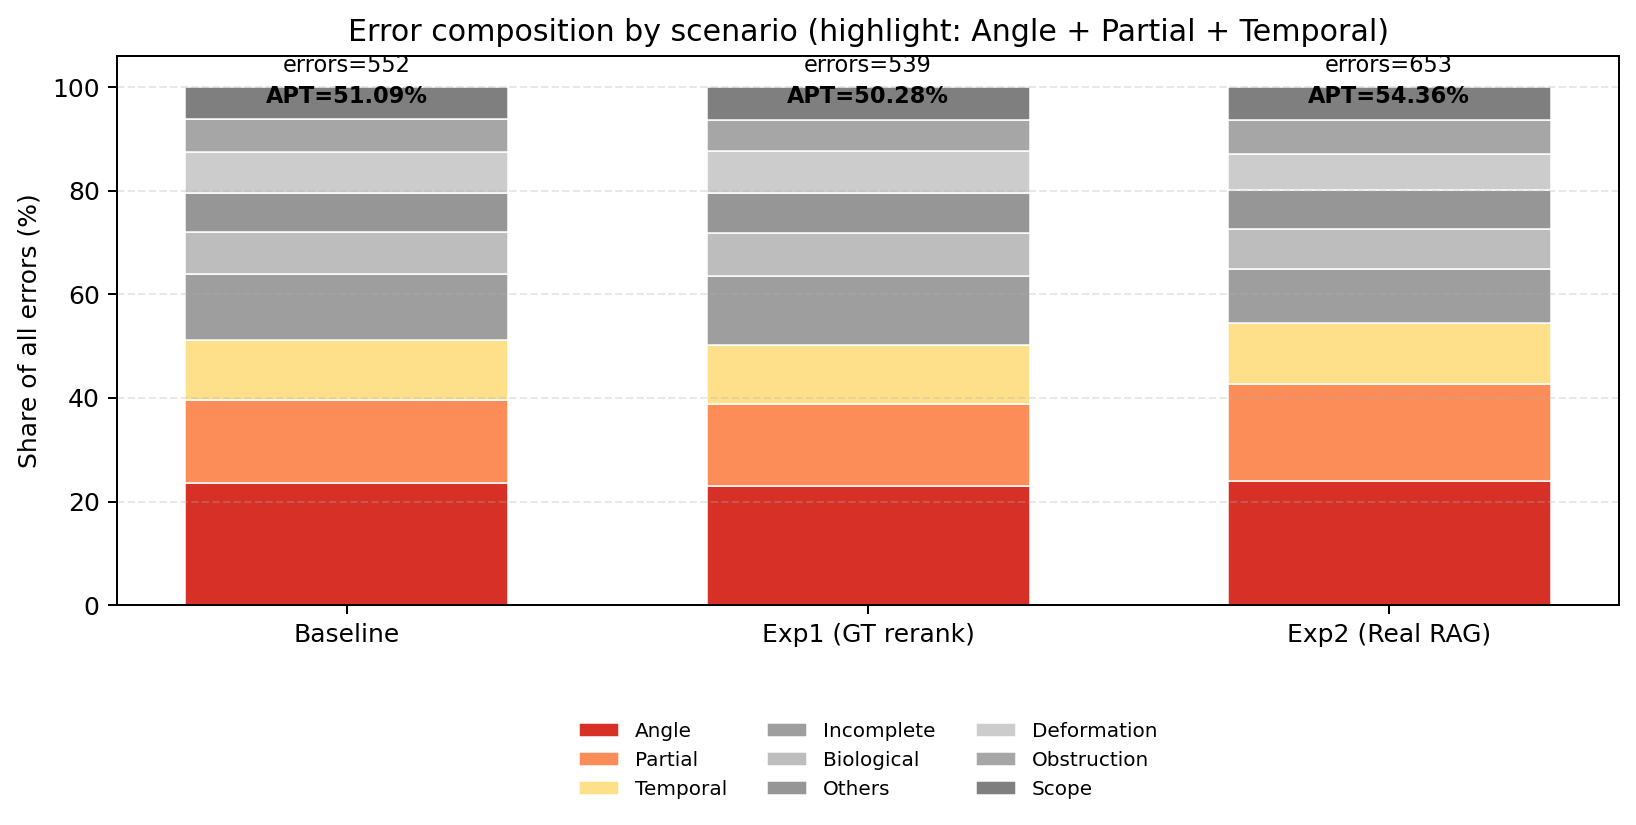
\includegraphics[width=\linewidth]{error_share_by_scenario_compare.png}
			\end{figure}
		\end{column}
		\begin{column}{0.36\textwidth}
			\begin{alertblock}{当前启发}
				\begin{itemize}
					\item 错误并非均匀分布，而是集中出现在若干困难场景。
					\item 难点主要落在 Temporal、Scope、Incomplete 等需要强视觉证据的场景。
					\item 后续应优先围绕这些场景优化 query 设计、召回策略和重排机制。
				\end{itemize}
			\end{alertblock}
		\end{column}
	\end{columns}
\end{frame}

\begin{frame}{研究进度与结果}
	\framesubtitle{当前分析与阶段结论}
	\begin{block}{阶段结论}
		\begin{itemize}
			\item 仅比较 overall accuracy 不足以解释 mRAG 流程，必须把“候选生成”和“候选排序”分开讨论。
			\item MagicLens 在固定候选集上的收益说明其具备一定的排序价值，但这还不等于完整检索能力已经解决。
		\end{itemize}
	\end{block}
	\begin{alertblock}{核心判断}
		\begin{itemize}
			\item 数据集给定候选与 GT 的低重叠率表明，真实 mRAG 的关键问题仍是如何从完整图像库中召回“有用证据”。
			\item 从 E1/E5、E3/E6、E3/E7 三组对照看，当前主要矛盾不在“是否加 MagicLens”，而在“给 MagicLens 什么候选、什么 instruction、它究竟做 rerank 还是 direct retriever 更合适”。
		\end{itemize}
	\end{alertblock}
\end{frame}

\section{后续计划与预期效果}
\subsection{实验计划}
\begin{frame}{后续计划与预期效果}
	\framesubtitle{后续的实验计划}
	\begin{columns}[T]
		\begin{column}{0.54\textwidth}
			\begin{block}{实验计划}
				\begin{enumerate}
					\item 完成 E6：在完整 corpus 上采用 CLIP 粗召回 + MagicLens 重排，验证主方案收益。
					\item 训练轻量级 prompt 生成模型，为 MagicLens 自动生成更适合检索的 query / instruction。
					\item 以“提升 GT 命中率、减少噪声候选、最终提升回答准确率”为目标，系统优化检索提示词设计。
					\item 对 Temporal、Scope、Incomplete 等困难场景开展消融分析，定位失败原因。
				\end{enumerate}
			\end{block}
		\end{column}
		\begin{column}{0.42\textwidth}
			\begin{alertblock}{进一步工作}
				\begin{itemize}
					\item 补充 No-RAG、w/o rerank 等控制实验，形成完整的证据链。
					\item 比较人工 prompt、规则模板与小模型生成 prompt 的差异，分析提示词与检索质量之间的关系。
					\item 探索扩散模型驱动的数据增强与检索器训练。
					\item 对比 E6 与 E7，判断 MagicLens 更适合作为 reranker 还是 direct retriever。
					\item 为后续具身/脑机接口应用奠定基础。
				\end{itemize}
			\end{alertblock}
		\end{column}
	\end{columns}
\end{frame}




\subsection{预期效果}
\begin{frame}{后续计划与预期效果}
	\framesubtitle{预期达到的效果}
	\begin{block}{预期研究结论}
		\begin{itemize}
			\item 证明多模态检索器相较于纯文本或弱检索策略具有明确收益。
			\item 定位完整 mRAG 中的主要性能瓶颈，判断其更偏向粗召回还是重排。
			\item 识别哪些类型的问题真正依赖视觉证据，形成面向后续优化的场景画像。
		\end{itemize}
	\end{block}
	\begin{alertblock}{预期成果形式}
		\begin{itemize}
			\item 一套可复现的 mRAG 检索评测流程与实验协议。
			\item MRAG-Bench 上系统性的检索器对比结果与错误分析。
			\item 形成一套面向 MagicLens 的提示词优化方法，为提升 GT 覆盖率、抑制噪声检索和改进最终回答效果提供实验基础。
		\end{itemize}
	\end{alertblock}
\end{frame}

\section{参考文献}
\begin{frame}[allowframebreaks]{参考文献}
	\scriptsize
	\setbeamertemplate{bibliography item}[text]
	\begin{thebibliography}{99}
		\bibitem{lewis2020}
		Lewis, P. et al. Retrieval-Augmented Generation for Knowledge-Intensive NLP Tasks. NeurIPS, 2020.
		\bibitem{gao2023}
		Gao, Y. et al. Retrieval-Augmented Generation for Large Language Models: A Survey. arXiv:2312.10997, 2023.
		\bibitem{mei2025}
		Mei, L. et al. A Survey of Multimodal Retrieval-Augmented Generation. arXiv:2504.08748, 2025.
		\bibitem{abootorabi2025}
		Abootorabi, M. M. et al. Ask in Any Modality: A Comprehensive Survey on Multimodal Retrieval-Augmented Generation. arXiv:2502.08826, 2025.
		\bibitem{radford2021}
		Radford, A. et al. Learning Transferable Visual Models From Natural Language Supervision. ICML, 2021.
		\bibitem{xie2025}
		Xie, C. et al. FG-CLIP: Fine-Grained Visual and Textual Alignment. arXiv:2505.05071, 2025.
		\bibitem{zhang2024longclip}
		Zhang, B. et al. Long-CLIP: Unlocking the Long-Text Capability of CLIP. arXiv:2403.15378, 2024.
		\bibitem{zhang2024magiclens}
		Zhang, K. et al. MagicLens: Self-Supervised Image Retrieval with Open-Ended Instructions. arXiv:2403.19651, 2024.
		\bibitem{hu2024}
		Hu, W. et al. MRAG-Bench: Vision-Centric Evaluation for Retrieval-Augmented Multimodal Models. arXiv:2410.08182, 2024.
	\end{thebibliography}
\end{frame}
\end{document}
